\chapter{Optimising Contur}
\label{chapterlabel5}

\section{Single Yoda Run}


\section{Grid Run}

For research purposes, contur users will in general be spending most of their time running contur on a grid as opposed to single yoda files. So focusing our optimisation efforts on the grid run is likely to produce more practical benefits for users. In addition we have two other motivations for focusing our efforts on optimising the grid run:

\begin{itemize}
\item There is more scope for achieving meaningful improvements in run time with the grid run. This viewpoint comes from observing from figure \ref{fig:single_yoda_start_profile_snakeviz} that the single yoda run time only takes around $20$ seconds, while from figure \ref{fig:grid_yoda_start_profile} we can see that the run time for smallish grid\footnote{The grid we are profiling contur on is $10 \times 10$, so contains $100$ yoda files, for research purposes it is common to run such a $10 \times 10$ grid across three different energy buckets ($7$,$10$ and $13$ TeV), which each bucket having $100$ yoda files for a total of $300$ yoda files. So the $20$ minutes we profiled for a single $10 \times 10$ would likely be close to an hour if run across the three energy buckets} takes up to $20$ minutes. Thus decreasing runtime for the single yoda by $50\%$ will only save us $10$ seconds in absolute terms, while the equivalent decrease for the grid run would save us $10$ minutes\footnote{Or $30$ minutes for the case where the grid has three energy buckets and $300$ yoda files.};
\item There is more scope for the grid run runtime to increase with changing research needs. The runtime for the grid run is highly dependent on the size of the grid used, as the grid grows in size so will the runtime. There is a practical limit how big a grid can be for contur resulting from this increasing runtime, in effect once a grid is so large it is too slow to run contur on it. Optimisation to the grid run that not only improve runtime on the current standard size grids but also reduce the speed that runtime increases with increasing runtime could have very practical benefits like making contur runs feasible on large grids where previously the run time was too slow;
\end{itemize}

For the above reasons the main focus of the optimisation from here on in will be on the grid run. From the dot plot in figure \ref{fig:grid_yoda_start_profile_dot} arising from the data produced from our initial grid profile we can see that grid runtime arises from two branches in the code flow, the first arising from the sort blocks method\footnote{See dark green box in dot plot}, which takes c.a. $25\%$ of runtime and the second being the likelihood calculation\footnote{sequence of boxes in the dot plot starting as yellow and morphing to green} which takes most of the remainder of the runtime. Our initial efforts will focus on making optimisation improvements for these two parts for the program.

\subsection{Sort Blocks}\label{sortBlocksSection}

\subsubsection{Background}
Before discussing the sort blocks method in detail it is first necessary to give some background into the flow of a contur grid run and where the sort blocks method sits within that flow. A grid run in contur is effectively just a group of single yoda runs performed within a loop with some slight differences\footnote{The most notable difference being in a single yoda contur run a large part of run time is spent reading in yoda files from Rivet with the background data. In the grid run this data reading is done for the first yoda file in the grid, but it is not necessary to repeat it for each new yoda file in the grid because the data read in for the first yoda file can be reused.}\footnote{The Depot class handles coordinating the contur run across the grid, the add point method in the Depot class used to run contur on individual yoda files in the grid}. So we can focus in on the operations contur performs on each yoda file it is passed in the grid. 

The yoda factories class in contur coordinates the run on each yoda file. When passed a yoda file yoda factories collects the data in the yoda file\footnote{The yoda file passed to yoda factories contains the signal events for the beyond standard model we are using contur to test} and the background experimental data needed to test against is also collected from Rivet\footnote{When running with theory option standard model simulated results will also be collected from Rivet}. The yoda file is composed of analysis objects, each analysis object is a histogram (is this correct? namely what I see as analysis object in the code is just another name for histogram) for which a confidence level can be calculated. The yoda factories class loops through these analysis objects, for each analysis object an instance of contur's likelihood class is created, the likelihood class compute the confidence level for the analysis object and stores it as its CLS attribute. The yoda factory performs this whole loop upon instantiation\footnote{This statement is true for our starting version of contur, as will be shown in \ref{sec:likelihood}, updates we will make for the likelihood optimisation will alter this flow} and stores a list of likelihood object\footnote{Each likelihood object in this list will have the confidence level for the analysis object it refers to stored in its CLS attribute} in its likelihood block attribute.

Yoda factories's sort blocks method is called after instantiation of a yoda factories object, so after all of the above calculations are carried out. Each likelihood object in yoda factories has collected has a pools attribute which gives the pool to which the analysis object used to create the likelihood object belongs. The sort blocks method simply buckets the likelihood objects by pool\footnote{So collects all the likelihood objects with the same pool into a single bucket}, and then for each pool it takes the likelihood object with the largest confidence level and discards the rest (Jon - please shout if this understanding is not correct).

\subsubsection{Changes made}
The profiling results in the dot plot in figure  \ref{fig:single_yoda_start_profile_snakeviz} are precise enough that we can pin point the major slow point in the sort blocks method to be the list comprehension in line 958 of yoda factories\footnote{This can also be easily picked up in the icicle plot when using Snakeviz's graphical viewer}. This list comprehension sits within a loop and the whole blocks of code looks as follows 


\begin{minted}{python}
for p in pools:
  if not p == omitted_pools:
    for item in like_blocks:
      if item.CLs == max([x.CLs for x in like_blocks if x.pools == p]) \
\end{minted}

In the above block of code the list comprehension in the last line is used to find the likelihood block in the pool with the largest confidence. The list comprehension on its own is not what makes the code slow, the list comprehension is placed within a nested for loop, which loops over pools and then within each pool iterate we have another loop over likelihood blocks. So in each yoda file the number of times we perform this list comprehension is the number of pools multiplied by the number of likelihood objects, and this is only for a single yoda file, across the whole grid we are doing this 100 times. Figure \ref{fig:list_comprehension} below shows that for our $10\times 10$ grid we are calling this list comprehension over a million times. So although each comprehension on its own takes less than $.002$ seconds this multiplied by a million still gives us a run time of over $200$ seconds.  

\begin{figure}[H]
\centering
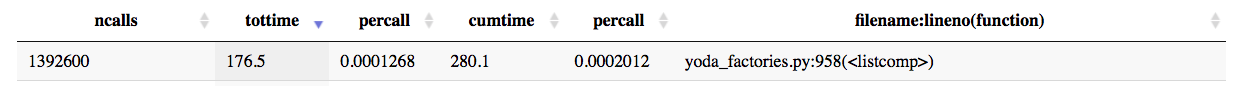
\includegraphics[scale=0.3]{plots/sort_blocks_list_comprehension.png}
\caption{List comprehension in sort blocks - Run time info}
\label{fig:list_comprehension}
\end{figure}

The optimisation change adopted here was to move the calculation of the max confidence level for each pool performed by the list comprehension outside of the nested for loop, thus reducing dramatically the number of times the calculation is performed. In its place we now only perform the calculation once per yoda file\footnote{So in our $10\times 10$  grid we go from perform the calculation over 1 million times to exactly $100$ times, once for each yoda file in the grid} and store the results in a dictionary whose key is the pool and value is the max confidence level for the pool. This dictionary is then used in place of the list comprehension in the above for loop. So within the nested for loop we have replaced a call to a list comprehension with a run time per call of $10^{-4}$ with a dictionary with a runtime per call\footnote{See https://towardsdatascience.com/faster-lookups-in-python-1d7503e9cd38} of $10^{-7}$, so the $10^6$ calls made in the loop will take $10^2$ seconds with our old implementation but only $10^{-1}$ seconds with the new implementation.

\subsubsection{Impact of changes}

Below we see the impact of the optimisation on the run time for the sort blocks method. In figure \ref{fig:sort_blocks_before} we can see that prior to optimisation the run time of the list comprehension is in line with our expectations from the previous section with a run time of $280$ seconds, order $10^2$ as expected and total run time\footnote{Remember the list comprehension is only part of the sort blocks method, not the whole of it so we will have additional run time from other parts of the method} for sort blocks is $293$ seconds While in figure \ref{fig:fig:sort_blocks_after} we see that we have a post optimisation run time of $7$ seconds for the whole of the sort blocks method. This run time would support the hypothesis that the run time for calling the dictionary in place of the list comprehension is of order $10^{-1}$ seconds and additional would suggest that the optimisation change made the calculation of the maximum confidence level for each pool slightly faster too, as prior to optimisation sort blocks had $13$ seconds of run time outside of the list comprehension, now after optimisation total run time is just $7$ seconds. 

\begin{figure}[H]
\centering

\includegraphics[scale=0.3]{plots/sort_blocks_before.png}
\caption{Sort blocks grid run time - Before optimisation}
\label{fig:sort_blocks_before}
\end{figure}



\begin{figure}[H]
\centering

\includegraphics[scale=0.3]{plots/sort_blocks_after.png}
\caption{Sort blocks grid run time - After optimisation}
\label{fig:sort_blocks_after}
\end{figure}



\subsection{Likelihood Calculation}\label{sec:likelihood}
\subsubsection{Background}
In the outline of the background for the sort blocks method in section \ref{sortBlocksSection} we touched on when the likelihood class comes into the flow of a contur run, namely how the yoda factory loops through all the analysis objects in the passed yoda file, instantiating a likelihood object for each analysis object which computes a confidence level. We however ignored the details of how these confidence levels are computed. We can see from the icicle plot in figure \ref{fig:grid_yoda_start_profile} that a material proportion of contur's run time is spent within the likelihood class\footnote{From the icicle plot we can see that out of a run time of around $1100$ seconds we spend $715$ seconds in the likelihood class calculations}.

Before outlining the steps taken to reduce the likelihood run time it is worth briefly outlining in greater detail the steps within the likelihood class to compute the confidence level for each analysis object. Upon instantiation the likelihood class computes two chi-square test statistics, a background and target test statistic (greater detail needs to be added here). These test statistics are then converted into p-values by assuming the test statistics are normally distributed and computing their survival function value\footnote{Defined by 1-cdf, so the area of the distribution to the right of the test statistic}. We use the sf method of the norm class found in scipy.stats to compute the p-values. Once a background and target p-values are computed they can be combined to calculate the confidence level for the analysis object.

Drilling down into the initial grid run profile results for the likelihood class we can see in figure \ref{fig:like_initial_profile} that the ts to pval method is where most of the run time is coming from in the likelihood object. This method computes p-values to test statistic and really just calls scipy.stats.norm.sf under the hood, so from here on we can focus our efforts on the scipy.stats.norm.sf method.

\begin{figure}[H]
\centering
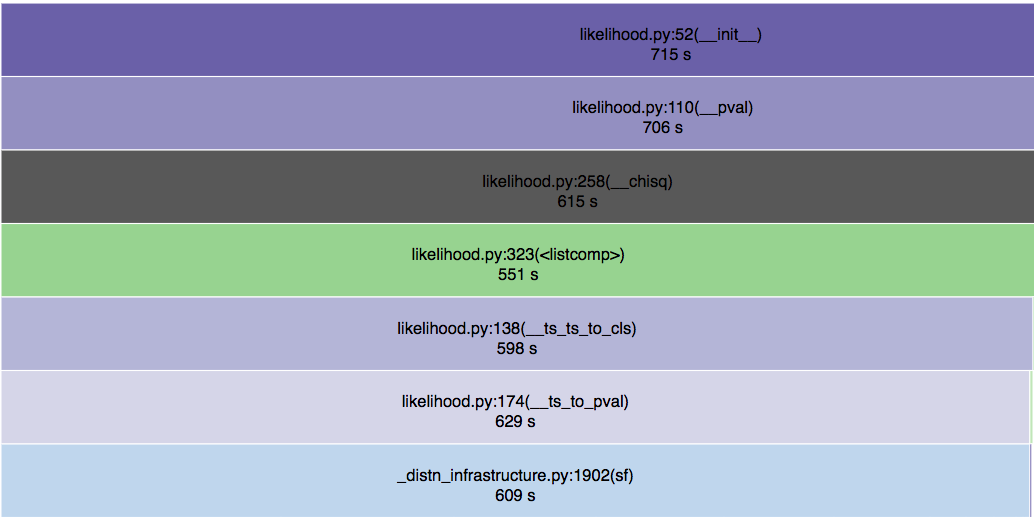
\includegraphics[scale=0.3]{plots/likelihood_drill_down.png}
\caption{Likelihood object - Initial profile}
\label{fig:like_initial_profile}
\end{figure}

From figure \ref{fig:ts_to_pval} below it becomes apparent that the large run time we observe from calling the survival function results from the large number of calls we make to the function. Each call to the survival function takes c.a. $0.0002$ seconds, but we make over $3$ million calls resulting in a total run of over $600$ seconds. 

\begin{figure}[H]
\centering
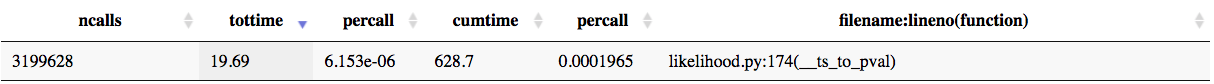
\includegraphics[scale=0.3]{plots/likelihood_count.png}
\caption{Likelihood object - ts to pval details}
\label{fig:ts_to_pval}
\end{figure}

\subsubsection{Scipy Survival Method}
From the previous section it should be clear that the survival function and reducing the number of times we call it is key to reducing the run time in the likelihood object. It is thus helpful to first understand better where the calls to the survival function arise when a likelihood class is instantiated. Within a likelihood object we get calls to the scipy survival function via the following routes:

\begin{itemize}
\item[1.] Every time the ts to pval method is called we have one call to survival function. Upon instantiation this method is called twice explicitly, giving us two calls to survival function ;
\item[2.]The ts ts to cls method calls ts to pval twice internally, so every time this method is called we have two calls to the survival function. The method is called once upon instantiation giving us two more calls to the survival function.;
\item[3.] The chisq method which computes the chi square test statistics will only call the survival function when an inverse for the covariance matrix of the analysis object cannot be computed\footnote{In the code the survival function will only be called when the condition "self.covBuilt and sb nuisance is not None" is false}. When the method calls the survival function the number of times it makes the calls is twice the number of buckets in the analysis object. So this is a minimum of $2$ calls but potentially much more than $2$ ;
\end{itemize}

From the above we see that each analysis object will have at least $4$ calls to the survival function\footnote{In practise it will be a lot more than this becuase of the chisq calls}, so across a whole yoda file the number of calls to the survival function will be at least $4$ multiplied by the number of analysis objects in the yoda file\footnote{For perspective here, the $10\times 10$ grid we profiled on had c.a. 60,000 likelihood objects created across $100$ yoda files suggesting on average each yoda file had $600$ valid analysis objects}. Finally we have $100$ yoda files in our grid, which need to be summed across to give the total number of calls we make to the survival function in our grid run.

To reduce the number of calls to the survival function we will adopt two approaches. The first is simple to check if we are making any unnecessary calls to the survival function anywhere that can easily be got rid of, this approach is simple but will not likely give high returns. The second approach is to take greater advantage of numpy's array functionality to see if via collecting test statistics into numpy arrays and passing these arrays of test statistics to the survival function, reducing the overall number of calls\footnote{So for example if we had four test statistics we wanted to pass to the survival function we would collect the test statistics into a single array and pass the array once to the survival function as opposed to four individual calls to the survival function}.

For the second approach to be effective we would require the run time for the survival function if passed a numpy array of length $n$ to be significantly less than the run if we just made $n$ separate calls to the survival function. We would expect this to be the case as the Scipy functions are built to enable fast array based computation on numpy arrays. Figure \ref{fig:loop_v_array} below shows the result of the profile we performed to test the performance of calling the survival function $n$ times within a loop or passing an array of length $n$ once. The $x$ axis gives the value of $n$ on the a log scale while the $y$ axis gives the run time for the loop (orange line) and the array (blue line) on a log scale. So from the plot we can see that our starting profile with $n$ between $10^6$-$10^7$ should give a run time between $10^2$-$10^3$ seconds which is in line with the c.a. $600$ seconds we actually observe.

\begin{figure}[H]
\centering
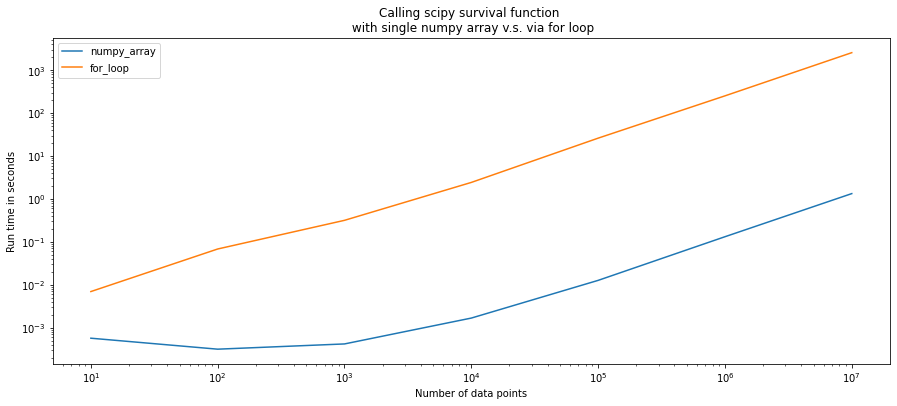
\includegraphics[scale=0.5]{plots/scipy_profile.png}
\caption{Scipy Survival Function - Loop vs Array}
\label{fig:loop_v_array}
\end{figure} 

\subsubsection{Changes made}
The optimisation changes to the likelihood calculation were made via multiple commits to the contur repository over the space of a couple weeks, they can be grouped into three groups of changes:

\begin{itemize}
\item[1.] Within likelihood objects making use of numpy arrays to reduce the number of calls to the survival function;
\item[2.] Within likelihood objects reducing unnecessary calls to the survival function;
\item[3.] Making use of numpy arrays to reduce the number of calls to the survival function across likelihood objects;
\end{itemize}

Of the above changes the first two are least disruptive in terms of their impact in overall flow of a contur run as they only make changes within the likelihood class. While the third change is more substantial as it alters the flow of a contur run between yoda factories and the likelihood class.

The first change\footnote{The change can be found in commit \href{https://gitlab.com/hepcedar/contur/-/commit/0b80789580cd0529bfdce28d2bae252755c45a63}{0b807895}} involves passing a tuple of background and signal test statistics to the ts to pval method and to the ts ts to cls methods, as opposed to passing the test statistics as separate calls. This reduces the calls to the survival function for these values from $4$ to $2$. In addition within the chisq method we also now pass a list of tuples of test statistics as opposed to making separate calls to the survival function. This ensures that whenever the chisq method makes on a call to the survival function it only makes $1$ call, so after all these changes, for analysis object we get at least $2$ calls to the survival function and at most $3$.

The second change\footnote{The change can be found in commit \href{https://gitlab.com/hepcedar/contur/-/commit/15ef923de401ced56f3186ed3bf6528c7d46f890}{15ef923d}} made is motivated from the observation that the ts ts to cls method has a call to ts to pval within it, so it computes the p value within the call. This is unnecessary as we have already computed the p value. The change introduce the pval to cls method which directly takes a p value and computes a confidence level from it. Negating the need to make another call to the survival function, so after this change we now have a minimum of $1$ call to the survival function and a maximum of $2$ in each analysis object.

From here on in let us simplify and assume that we have exactly $2$ calls to the survival function for each analysis object and for each yoda file we have $m$ analysis objects. So in a grid with $n$ yoda files after the above changes we have $2\times n\times m$ calls to the survival function. So on our $100$ yoda file grid assuming $m=600$ this will still give us 120,000 calls to the survival function. Additionally we can see with an expanding grid size this number of calls will grow, for example with 1,000 yoda files the number of calls to the survival function will be above 1 million again. So the current configuration is not robust against future increases in grid size which may be used by contur. The final set of optimisation changes we will make will resolve this issue by getting rid of the run time dependence on $m$.

To achieve this, let us first remind ourselves how the the current set up works. Upon instantiation of the yoda factories class we loop through all analysis objects instantiating a likelihood object for each and doing the full likelihood calculation (i.e. computing the confidence level) upon instantiation of the class. So at the end of this process we have a yoda factory object with a likelihood blocks attribute that contains all the likelihood objects. This process can be split into steps that allow us eliminate dependence on the number of analysis objects. This can be done by instead of using the survival function within the likelihood object, we can instead just collect test statistics in the likelihood object which can then be collected into a numpy array in yoda factories composed of test statistics from all the likelihood objects, this array can then be passed once the survival function.

Implementing this change in practise is spread across two commits\footnote{The first commit \href{https://gitlab.com/hepcedar/contur/-/commit/299b03a86812b47e30ed66d4f82a59a3584cf523}{299b03a8} introduces the likelihood blocks ts to cls function, while the second commit \href{https://gitlab.com/hepcedar/contur/-/commit/2769e1c2a020efd2de2919db2413309eef8a8e64}{2769e1c2} introduces the likelihood blocks find dominant ts function }. 

For the first commit we introduce the likelihood blocks ts to cls function, which takes a list of likelihood blocks and computes a confidence level for each likelihood block in the list. In terms of the flow of contur, with this change we alter the likelihood object so it no longer calculates the confidence level upon instantiation, so when we instantiate yoda factories we now have a list of likelihood objects in the likelihood blocks attribute with just test statistics not confidence level, we pass this list to the new function which does the confidence level calculation. After this change we will $n + (n\times m)$ calls to the survival function.

For the second commit we introduce the likelihood blocks find dominant ts function. This function finds the chi square test statistic in an analysis object that gives the largest confidence when the covariance matrix does not have a valid inverse. Thus it moves the calls to the survival function that take place within the chisqr method into a single call in yoda factories. After this change the number of calls to the survival function will be $2n$ so we have removed the dependence on $m$ of the number of calls.

\subsubsection{Impact of changes}

The impact of the optimisation on the run time for the likelihood class and the associated new functions can be seen in figure \ref{fig:like_last_profile} below. From the figure we can see that impact of the optimisation on the run time for the confidence level calculation has been substantial, from a starting run time of c.a. $600$ seconds the optimisation has reduced the total run time to just below $20$ seconds.

\begin{figure}[H]
\centering
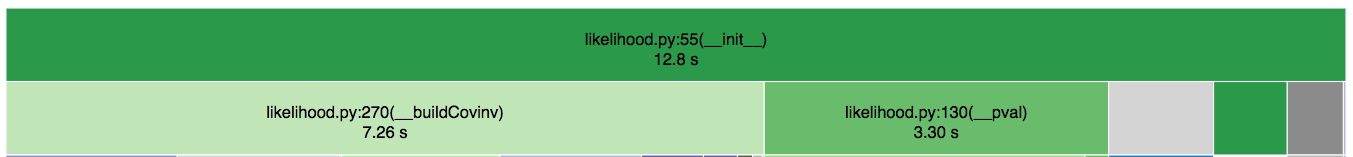
\includegraphics[scale=0.3]{plots/like_after_change.png}

\includegraphics[scale=0.3]{plots/like_ts_to_cls.png}

\includegraphics[scale=0.3]{plots/like_blocks_find_dominant_ts.png}
\caption{Likelihood object and new functions - Profile after optimisation}
\label{fig:like_last_profile}
\end{figure} 








